\section{Auswertung}
\label{sec:Auswertung}
Sämtliche im Folgenden durchgeführten Ausgleichsrechnungen werden mit der \emph{curve fit} Funktion aus dem für \emph{Python} geschriebenen package \emph{NumPy}\cite{scipy} durchgeführt. Fehlerrechnungen werden mit dem für \emph{Python} geschriebenen package \emph{Uncertainties}\cite{uncertainties} ausgeführt.

\subsection{Allgemeine Auswertung der Filmstreifen}
\label{sec:allgemein}
Zur Auswertung wird der Nullpunkt in die Mitte des linken ausgestanzten Loches gesetzt, da in diesem Punkt der Strahl die Kamera verlässt. Somit entspricht der Abstand zwischen beiden ausgestanzten Löchern einem Winkel von $\theta=\SI{90}{\degree}$. Der Abstand der Streifen zum Nullpunkt werden mit einem Geodreik vermessen und mit der Beziehung
\begin{align}
	\theta=\frac{s}{2R}
\end{align}
in den Beugungswinkel überführt. Dabei beschreibt $s$ den Abstand des auftretenen Reflex zum Nullpunkt und $R=\SI{5.73}{\centi\meter}$ den Radius der verwendeten Kamera.  Aufgrund der Fehleranfälligkeit beim ablesen, wird auf jeden Reflex ein Unsicherheit  $\Delta s=\SI{1}{\milli\meter}$ angenommen.

\subsection{Metallprobe}
Die im vorherigen Kapitel beschriebenen Messgrößen und der Netzebenenabstand $d$, welcher mit der Bragg-Bedingung XXX bestimmt wird, sind in Tabelle \ref{table:A1} für die verwendete Metallprobe 9 zusammengefasst.
\begin{table}
    \centering
    \caption{Messdaten der Metallprobe.}
    \label{table:A1}
    \sisetup{parse-numbers=false}
    \begin{tabular}{
	S[table-format=2.1]
	@{${}\pm{}$}
	S[table-format=1.1, table-number-alignment = left]
	S[table-format=1.3]
	@{${}\pm{}$}
	S[table-format=1.3, table-number-alignment = left]
	S[table-format=1.3]
	@{${}\pm{}$}
	S[table-format=1.3, table-number-alignment = left]
	}
	\toprule
	\multicolumn{2}{c}{$s\:/\: \si{\centi\meter}$}		& \multicolumn{2}{c}{$\theta\:/\: \si{\centi\meter}$}		&
    \multicolumn{2}{c}{$d \:/\: \si{\angstrom}$}		\\ 
	\midrule
    4.0  & 0.1 & 0.349 & 0.009 & 2.25   & 0.05   \\
5.7  & 0.1 & 0.497 & 0.009 & 1.62   & 0.03   \\
7.1  & 0.1 & 0.620 & 0.009 & 1.33   & 0.02   \\
8.4  & 0.1 & 0.733 & 0.009 & 1.15   & 0.01   \\
9.6  & 0.1 & 0.838 & 0.009 & 1.037  & 0.008  \\
10.9 & 0.1 & 0.951 & 0.009 & 0.947  & 0.006  \\
12.2 & 0.1 & 1.065 & 0.009 & 0.881  & 0.004  \\
13.8 & 0.1 & 1.204 & 0.009 & 0.826  & 0.003  \\
16.2 & 0.1 & 1.414 & 0.009 & 0.780  & 0.001  \\
16.4 & 0.1 & 1.435 & 0.009 & 0.7795 & 0.0009 \\

    \bottomrule
    \end{tabular}
    \end{table}

Die letzten beiden Einträge in der Tabelle stehen aus einer Ringaufspaltung. Bei der Betrachtung der Netzebenenabstände $d$ für die Ringaufspaltung, ist zu erkennen, dass sich diese erst in der dritten Nachkommerstelle unterscheiden. Zudem liegt der eine Wert im Fehlerintervall des anderen und umgekehrt. Aufgrund dessen werden im Folgenden die beiden Abstände gemittelt und mit der mittleren Wellelänge der $K_\alpha$-Linie ein gemittelter Netzebenenabstand berechnet. \\

Zur Bestimmung der Kristallstruktur wird das Verhältnis
\begin{align}
	\frac{d_1}{d_i}=\frac{m_i}{m_1}
	\label{eq:dm}
\end{align}
verwendet, wobei gilt $m=\sqrt{h^2+k^2+l^2}$. Dadurch erfolgt ein Vergleich der Theorie (rechte Seite) mit den experimentell bestimmten Werten (linke Seite).
In Tabelle \ref{table:A2} sind die ersten neun Reflexe der Kristallstrukturen simple-cubic (sc), body centered cubic (bbc), face centered cubic (fcc) und Diamant aufgelistet. Zudem wird das in Gleichung \ref{eq:dm} beschriebene Verhältnis gebildet, um dieses mit der Probe zu vergleichen.

\begin{table}
    \centering
    \caption{Vergleich der Verhältnisse für die Metallprobe.}
    \label{table:A2}
    \sisetup{parse-numbers=false}
    \begin{tabular}{
	S[table-format=3.0]
	S[table-format=1.2]
	S[table-format=3.0]
	S[table-format=1.2]
	S[table-format=3.0]
	S[table-format=1.2]
	S[table-format=3.0]
	S[table-format=1.2]
	S[table-format=1.2]
	@{${}\pm{}$}
	S[table-format=1.2, table-number-alignment = left]
	}
	\toprule
	{$\text{sc}$}		& {$\left(\frac{m_i}{m_1}\right)_{sc}$}		& 
	{$\text{bcc}$}		& {$\left(\frac{m_i}{m_1}\right)_{bcc}$}		& 
	{$\text{fcc}$}		& {$\left(\frac{m_i}{m_1}\right)_{fcc}$}		& 
	{$\text{diamant}$}		& {$\left(\frac{m_i}{m_1}\right)_{dia}$}		& 
	\multicolumn{2}{c}{$\frac{d_1}{d_i}$}		\\ 
	\midrule
    100 & 1.00 & 110 & 1.00 & 111 & 1.00 & 111 & 1.00 & 1.0  & 0    \\
110 & 1.41 & 200 & 1.41 & 200 & 1.15 & 220 & 1.63 & 1.40 & 0.04 \\
111 & 1.73 & 211 & 1.73 & 220 & 1.63 & 311 & 1.91 & 1.70 & 0.05 \\
200 & 2.00 & 220 & 2.00 & 311 & 1.91 & 400 & 2.31 & 1.96 & 0.05 \\
210 & 2.24 & 310 & 2.24 & 222 & 2.00 & 331 & 2.52 & 2.17 & 0.05 \\
211 & 2.45 & 222 & 2.45 & 400 & 2.31 & 422 & 2.83 & 2.38 & 0.06 \\
220 & 2.83 & 321 & 2.65 & 331 & 2.52 & 333 & 3.00 & 2.56 & 0.06 \\
221 & 3.00 & 400 & 2.83 & 420 & 2.58 & 440 & 3.27 & 2.73 & 0.07 \\
310 & 3.16 & 330 & 3.00 & 422 & 2.83 & 531 & 3.42 & 2.90 & 0.07 \\

    \bottomrule
    \end{tabular}
    \end{table}


Anhand der absoluten Zahlen kann zunächst die Aussage getroffen werden, dass die Diamantstruktur nicht der gesuchten Kristallprobe entspricht. Um die anderen Strukturen bewerten zu können, wird in Tabelle \ref{table:A3} die absolute Abweichung in Prozent angegeben.

\begin{table}
    \centering
    \caption{Vergleich der Verhältnisse mit zusätzlicher Abweichung.}
    \label{table:A3}
    \sisetup{parse-numbers=false}
    \begin{tabular}{
	S[table-format=1.2]
	S[table-format=2.2]
	S[table-format=1.2]
	S[table-format=1.2]
	S[table-format=1.2]
	S[table-format=2.2]
	S[table-format=1.2]
	@{${}\pm{}$}
	S[table-format=1.2, table-number-alignment = left]
	}
	\toprule
	{$\left(\frac{m_i}{m_1}\right)_{sc}$}		& {$|Abw_{sc}|\:/\: \si{\percent}$}		& 
	{$\left(\frac{m_i}{m_1}\right)_{bcc}$}		& {$|Abw_{bcc}|\:/\: \si{\percent}$}		& 
	{$\left(\frac{m_i}{m_1}\right)_{fcc}$}		& {$|Abw_{fcc}|\:/\: \si{\percent}$}		& 
	\multicolumn{2}{c}{$\frac{d_1}{d_i}$}		\\ 
	\midrule
    1.00 & 0.00  & 1.00 & 0.00 & 1.00 & 0.00  & 1.0  & 0    \\
1.41 & 1.37  & 1.41 & 1.37 & 1.15 & 17.23 & 1.40 & 0.04 \\
1.73 & 2.01  & 1.73 & 2.01 & 1.63 & 3.82  & 1.70 & 0.05 \\
2.00 & 2.23  & 2.00 & 2.23 & 1.91 & 2.12  & 1.96 & 0.05 \\
2.24 & 2.91  & 2.24 & 2.91 & 2.00 & 7.95  & 2.17 & 0.05 \\
2.45 & 2.90  & 2.45 & 2.90 & 2.31 & 2.98  & 2.38 & 0.06 \\
2.83 & 10.60 & 2.65 & 3.46 & 2.52 & 1.59  & 2.56 & 0.06 \\
3.00 & 9.90  & 2.83 & 3.62 & 2.58 & 5.41  & 2.73 & 0.07 \\
3.16 & 9.32  & 3.00 & 3.71 & 2.83 & 2.22  & 2.89 & 0.07 \\

    \bottomrule
    \end{tabular}
    \end{table}


Zu beobachten ist, dass die bcc-Kristallstruktur kontinuierlich nur geringe Abweichungen unter $\SI{4}{\percent}$ aufweißt. Somit wird angenommen, dass die Probe eine bcc-Struktur besitzt.

Desweiteren ist die Gitterkonstante $a$ der Probe zu bestimmen. Diese wird nach Gleichung XXX berechnet und in Abbildung \ref{fig:plot1} gegen $\cos^2{(\theta)}$ aufgetragen. Durch die verwendete lineare Ausgleichsrechnung
\begin{align}
	a(\cos{(\theta)})= b\cos^2{(\theta)} + c
	\label{eq:FIT}
\end{align}

\begin{figure}
  \centering
  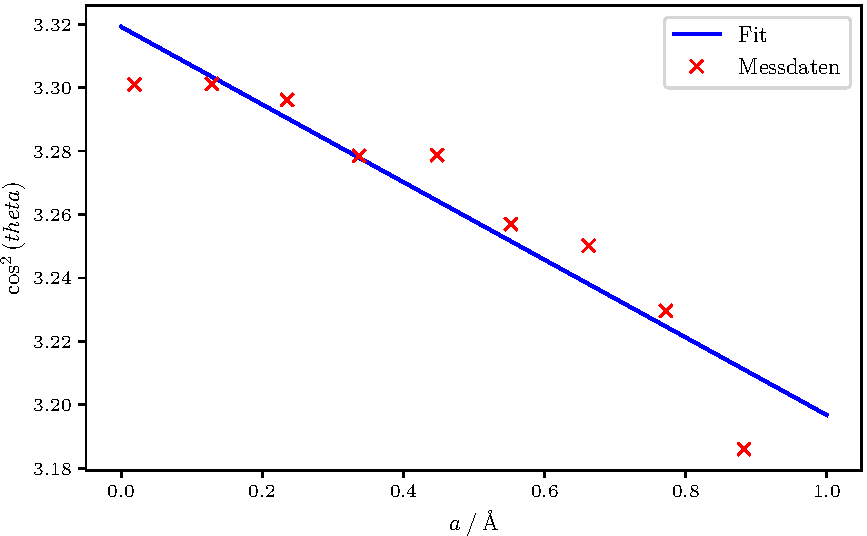
\includegraphics[scale=0.75]{build/Metall.pdf}
  \caption{Messdaten und Fitergebnis.}
  \label{fig:plot1}
\end{figure}

werden die in Kapitel XXX angesprochenen systematischen Fehler korrigiert. Die resultierenden Fitparamter lauten:
\begin{align}
	b&= \SI{-0.125+-0.016}{\angstrom}
 \\
	c&= \SI{3.3192+-0.0087}{\angstrom}

\end{align}

Die Gitterkonstante und die vorliegende bcc-Struktur weißt nach \cite{gitter} auf Niob hin. Die Abweichung zur der in der Literatur angegebenen Gitterkonstante
$a=\SI{3.30}{\angstrom}$ beträgt $\SI{1.038+-0.005}{\percent}
$.

\subsection{Salzprobe}
Die Salzprobe muss eine Gitterstruktur aufweisen, die aus zwei verschiedenen Atomen besteht. Nach \cite{skript} werden somit die Zinkblenden-, die Steinsalz, Cäsiumchlorid- und Fluoritstruktur im folgenden untersucht. Dafür werden mit Gleichung XXX alle aufkommenden Reflexe ermittelt. Da das Material unbekannt ist, lässt sich keine Aussagen über den Atomformfaktor $f$ treffen. Aus diesem Grund werden die beiden jeweiligen Untergitter der zuvor genannten Gitterstrukturen untersucht. Tritt also ein Reflex in einem der Untergitter auf, wird dieser zu den Reflexen der Gesamtstruktur hinzugezählt. Diese Methode funktioniert nicht bei der Cäsiumchlorid-Struktur, da dessen Elementarzelle nur zwei Atome besitzt und zusätzlich einer der Koordinaten $(0,0,0)$ ist. Somit würde bei jeder Kombination von Millerindizes ein Reflex entstehen. Deshalb wird zur Vereinfachung angenommen:
\begin{align}
	f_1\approx f_2
\end{align} 

Die auf dem Filmstreifen vermessenen Reflexe, die sich daraus ergebenen Winkel $\theta$ und die Netzebenenabstände sind in Tabelle \ref{table:A4} aufgelistet.

\begin{table}
    \centering
    \caption{Messdaten der Salzprobe.}
    \label{table:A4}
    \sisetup{parse-numbers=false}
    \begin{tabular}{
	S[table-format=2.2]
	S[table-format=1.2]
	S[table-format=1.2]
	}
	\toprule
	{$s\:/\: \si{\centi\meter}$}		& {$\theta$}		& 
	{$d \:/\: \si{\angstrom}$}		\\ 
	\midrule
    2.75  & 0.24 & 3.24 \\
3.90  & 0.34 & 2.31 \\
4.80  & 0.42 & 1.90 \\
5.60  & 0.49 & 1.64 \\
6.30  & 0.55 & 1.48 \\
7.00  & 0.61 & 1.34 \\
8.30  & 0.72 & 1.16 \\
8.90  & 0.78 & 1.10 \\
9.55  & 0.83 & 1.04 \\
10.20 & 0.89 & 0.99 \\
11.55 & 1.01 & 0.91 \\
12.20 & 1.06 & 0.88 \\
12.80 & 1.12 & 0.86 \\
14.10 & 1.23 & 0.82 \\
14.90 & 1.30 & 0.80 \\
16.50 & 1.44 & 0.78 \\

    \bottomrule
    \end{tabular}
    \end{table}


Zur Auswertung wird für jeweils alle dreizehn Reflexe auf dem Filmstreifen  und alle möglichen Millerindizes die Gitterkonstante $a$ berechnet. Stimmt die angenommene Gitterstruktur mit der Gitterstruktur der Probe überein, ist die Gitterkonstante $a$ in einer Diagonale durchgehend zu finden. Da die Zinkblenden-, die Steinsalz  und Fluoritstruktur die gleichen Reflexe aufweisen, sind diese zusammen in Abbildung \ref{fig:C_excel} und die  Cäsiumchloridstruktur in Abbildung \ref{fig:A_excel} dargestellt.

\begin{figure}
	\centering
	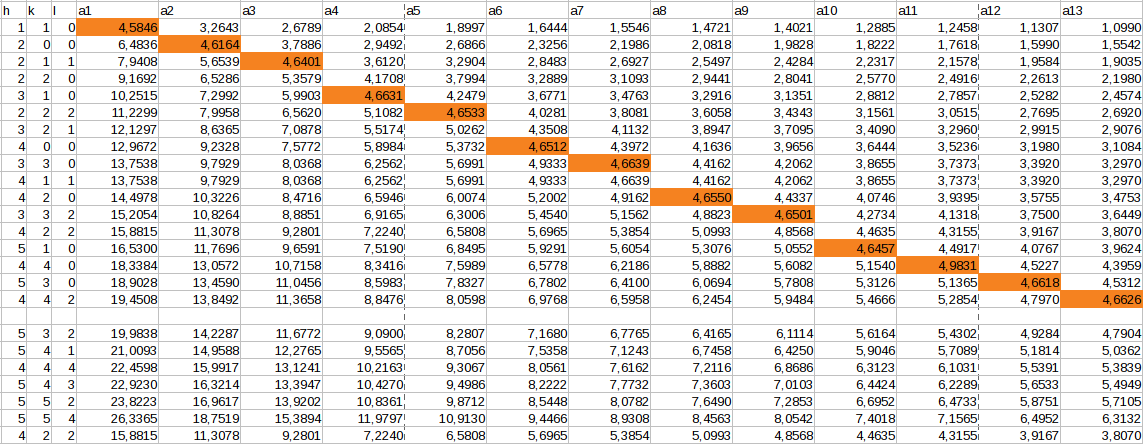
\includegraphics[angle=90,scale=0.75]{ressources/Caesiumchlorid.png}
	\caption{Messdaten und Fitergebnis.}
    \label{fig:C_excel}
\end{figure}


\begin{figure}
	\centering
	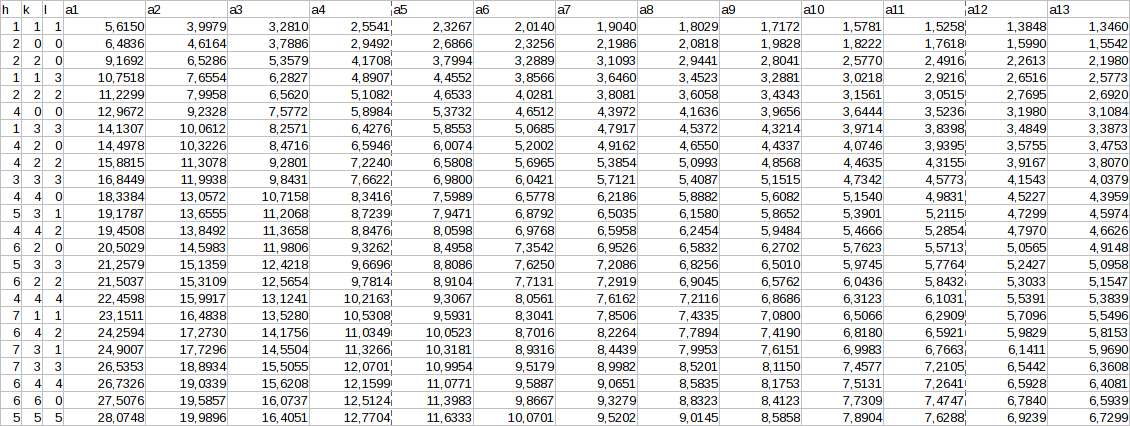
\includegraphics[angle=90,scale=0.75]{ressources/Strukturen.png}
	\caption{Messdaten und Fitergebnis.}
    \label{fig:A_excel}
\end{figure}

Bei dem Vergleich von Abbildung \ref{fig:C_excel} und \ref{fig:A_excel} ist zuerkennen, dass die Salzprobe eine Cäsiumchloridstruktur besitzt. Zur Korrektur der systematischen Fehler wird erneut die Gitterkonstante $a$ gegen $\cos^2{\theta}$ aufgetragen und eine lineare Ausgleichsrechung \eqref{eq:FIT} vorgenommen. Es ist anzumerken, dass der in Abbildung \ref{fig:plot5} grün markierte Messwert nicht in die lineare Ausgleichrechnung mit eingeht.

\begin{figure}
	\centering
	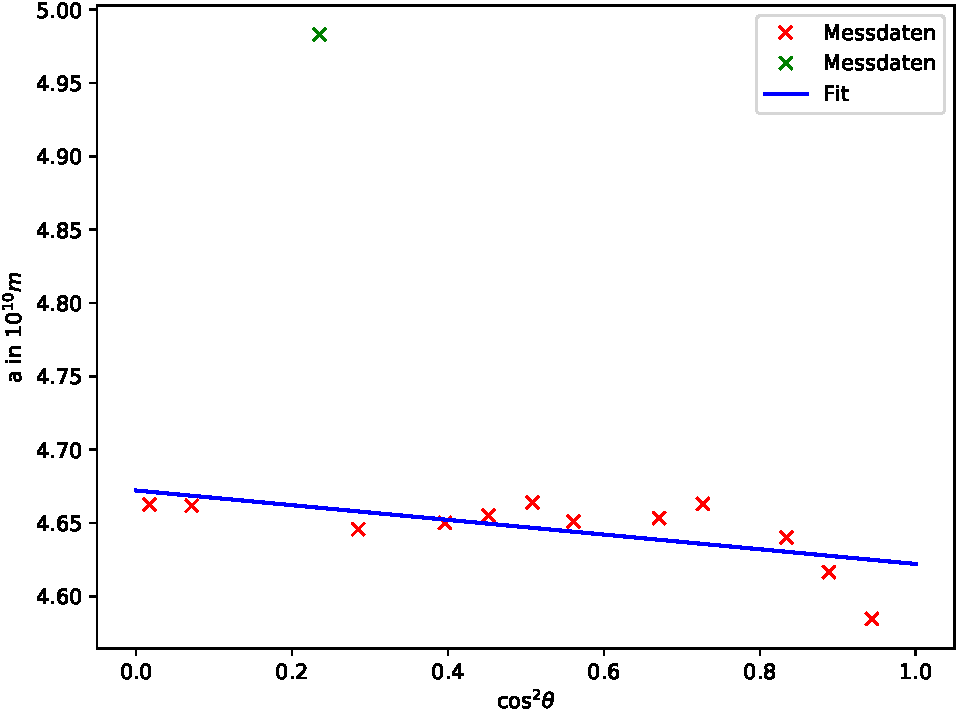
\includegraphics[scale=0.75]{build/Salz.pdf}
	\caption{Messdaten und Fitergebnis.}
    \label{fig:plot5}
\end{figure}

Die Ergebnisse der Fitparamter lauten:

\begin{align}
	b&= \SI{-0.050+-0.019}{\angstrom}
 \\
	c&= \SI{4.672+-0.011}{\angstrom}

\end{align}





% % Examples
% \begin{equation}
%   U(t) = a \sin(b t + c) + d
% \end{equation}
%
% \begin{align}
%   a &= \input{build/a.tex} \\
%   b &= \input{build/b.tex} \\
%   c &= \input{build/c.tex} \\
%   d &= \input{build/d.tex} .
% \end{align}
% Die Messdaten und das Ergebnis des Fits sind in Abbildung~\ref{fig:plot} geplottet.
%
% %Tabelle mit Messdaten
% \begin{table}
%   \centering
%   \caption{Messdaten.}
%   \label{tab:data}
%   \sisetup{parse-numbers=false}
%   \begin{tabular}{
% % format 1.3 bedeutet eine Stelle vorm Komma, 3 danach
%     S[table-format=1.3]
%     S[table-format=-1.2]
%     @{${}\pm{}$}
%     S[table-format=1.2]
%     @{\hspace*{3em}\hspace*{\tabcolsep}}
%     S[table-format=1.3]
%     S[table-format=-1.2]
%     @{${}\pm{}$}
%     S[table-format=1.2]
%   }
%     \toprule
%     {$t \:/\: \si{\milli\second}$} & \multicolumn{2}{c}{$U \:/\: \si{\kilo\volt}$\hspace*{3em}} &
%     {$t \:/\: \si{\milli\second}$} & \multicolumn{2}{c}{$U \:/\: \si{\kilo\volt}$} \\
%     \midrule
%     \input{build/table.tex}
%     \bottomrule
%   \end{tabular}
% \end{table}
%
% % Standard Plot
% \begin{figure}
%   \centering
%   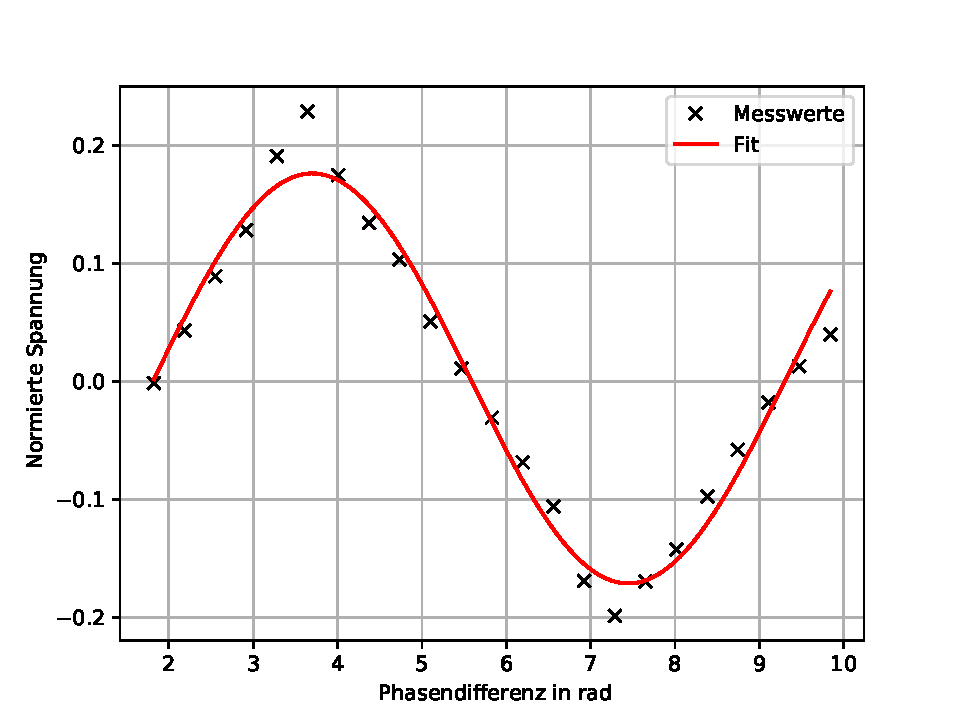
\includegraphics{build/plot.pdf}
%   \caption{Messdaten und Fitergebnis.}
%   \label{fig:plot}
% \end{figure}
%
% 2x2 Plot
% \begin{figure*}
%     \centering
%     \begin{subfigure}[b]{0.475\textwidth}
%         \centering
%         \includegraphics[width=\textwidth]{Abbildungen/Schaltung1.pdf}
%         \caption[]%
%         {{\small Schaltung 1.}}
%         \label{fig:Schaltung1}
%     \end{subfigure}
%     \hfill
%     \begin{subfigure}[b]{0.475\textwidth}
%         \centering
%         \includegraphics[width=\textwidth]{Abbildungen/Schaltung2.pdf}
%         \caption[]%
%         {{\small Schaltung 2.}}
%         \label{fig:Schaltung2}
%     \end{subfigure}
%     \vskip\baselineskip
%     \begin{subfigure}[b]{0.475\textwidth}
%         \centering
%         \includegraphics[width=\textwidth]{Abbildungen/Schaltung4.pdf}    % Zahlen vertauscht ... -.-
%         \caption[]%
%         {{\small Schaltung 3.}}
%         \label{fig:Schaltung3}
%     \end{subfigure}
%     \quad
%     \begin{subfigure}[b]{0.475\textwidth}
%         \centering
%         \includegraphics[width=\textwidth]{Abbildungen/Schaltung3.pdf}
%         \caption[]%
%         {{\small Schaltung 4.}}
%         \label{fig:Schaltung4}
%     \end{subfigure}
%     \caption[]
%     {Ersatzschaltbilder der verschiedenen Teilaufgaben.}
%     \label{fig:Schaltungen}
% \end{figure*}
